\section{Casi reali: ricostruzione degli episodi}
\label{sec:episodi}

% Persone 2 e 3 — circa 1 pagina complessiva.
\subsection{chalk/debug, 8 settembre 2025}
% Persona 2 — circa 0,5 pagina.
\subsubsection{Cronologia essenziale e componenti coinvolti}

L'8 settembre 2025 l'account npm del manutentore fu usato per pubblicare
versioni sospette, tra cui \texttt{chalk@5.6.1} e \texttt{debug@4.4.2}.
Aikido segnalò l'attività anomala alle 13:16 UTC; poco dopo il manutentore
confermò di aver perso il controllo dell'account e i repository GitHub
avvisarono di non usare le versioni coinvolte~\cite{aikido2025,chalk2025}.

\begin{figure}[H]
    \centering
    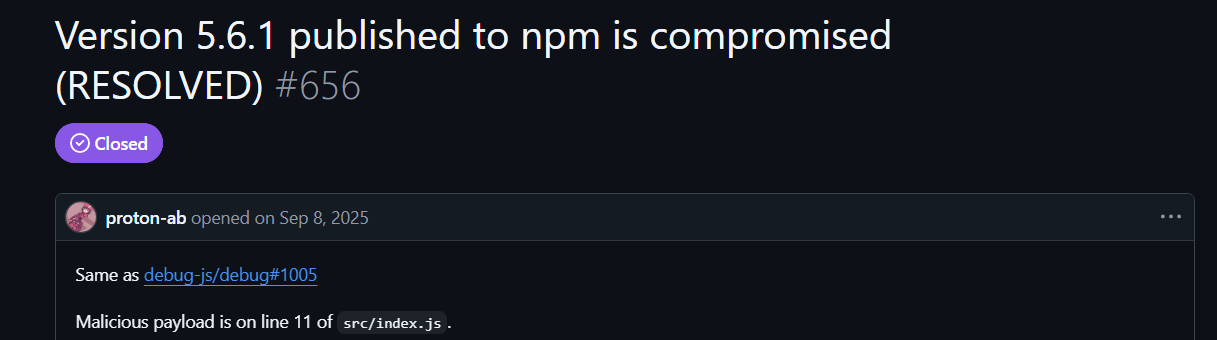
\includegraphics[width=0.78\textwidth]{immagine_compromesso_chalk.png}
    \caption{Segnalazione della versione compromessa di chalk su GitHub.}
    {\footnotesize Fonte: \cite{chalk2025}\par}
    \label{fig:issue-chalk-compromesso}
\end{figure}

\subsubsection{Risposta adottata}

Le versioni compromesse furono rimosse da npm. L'advisory raccomandò di
aggiornare alle versioni corrette e, se quelle malevole erano state installate,
di rimuovere le dipendenze scaricate e ricostruire da zero i bundle browser
potenzialmente contaminati~\cite{debug2025}. Le misure preventive sono
discusse nel capitolo~\ref{sec:mitigazioni}.

\subsection{AUR, segnalazione del 12 giugno 2026}
\label{subsec:aur-episodio}
% Persona 3 — circa 0,5 pagina.
\subsubsection{Esempio e cronologia essenziale}
L'11 giugno 2026 fu segnalata una modifica sospetta a
\texttt{gnome-randr-rust}: un nuovo manutentore aveva aggiunto uno script
che installava la dipendenza npm \texttt{atomic-lockfile}, non pertinente al
software~\cite{aur-mail-gnome-randr}. Il giorno dopo Arch confermò un'ondata
di adozioni e aggiornamenti malevoli e invitò a controllare le modifiche a
\texttt{PKGBUILD} e agli script d'installazione
~\cite{arch-aur-incident-2026}.

\subsubsection{Evidenze disponibili e risposta}
Un manutentore AUR confermò la natura malevola del commit, ripristinò la
revisione precedente e sospese l'account responsabile
~\cite{aur-mail-gnome-randr}. Arch spiegò che stava rintracciando i commit
malevoli e cercando di impedire nuove modifiche
~\cite{arch-aur-incident-2026}. Questi interventi documentano la risposta sul
repository, ma non provano installazioni o vittime; il singolo esempio non va
esteso automaticamente all'intera ondata.
